\documentclass[10pt, xcolor=table]{beamer}

\usetheme{m}

\usepackage{times}
\usepackage{tikz}
\usepackage{amsmath}
\usepackage{fancyvrb}
\usepackage{xspace}

\usepackage{booktabs}
\usepackage[scale=2]{ccicons}

%\usepackage{pgfplots}
%\usepgfplotslibrary{dateplot}

\usepackage{listings}

\usepackage[latin1]{inputenc}
\usepackage[spanish]{babel}


\title{}
\subtitle{�rboles C4.5, C5.0 y Random Forest}
\date{}
\author{Luis Mar�a Costero Valero\\Jes�s Javier Dom�nech Arellano}
\institute{Enero 2016}

\titlegraphic{\hfill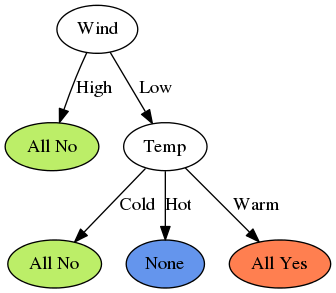
\includegraphics[scale=0.2]{images/portada.png}}

\definecolor{bgg}{HTML}{FBFBFB}
\def\gcolor{bgg}    % while presenting
%\def\gcolor{black} % while developing

\def\tikzpicdim{
  \draw[step=0.1cm, color=\gcolor] (0,-1) grid (12,7);
  \draw[step=1cm, color=\gcolor] (0,-1) grid (12,7);
}

\let\tikzpicdimlarge\tikzpicdim


\metroset{inner/sectiontitleformat=regular}
\metroset{outer/frametitleformat=regular}
\metroset{block=fill}

\newcommand\sectionDark[1]{{\metroset{background=dark} \section{#1} }}
\begin{document}

\maketitle


%%======= INDICE ========================================
\begin{frame}
  \frametitle{�ndice}
  \setbeamertemplate{section in toc}[sections numbered]
  \tableofcontents
\end{frame}


%=================================================
\sectionDark{ID3}
%=================================================
\begin{frame}
  \frametitle{TDIDT\footnote{Diapositiva sacada del temario de SGDI}}
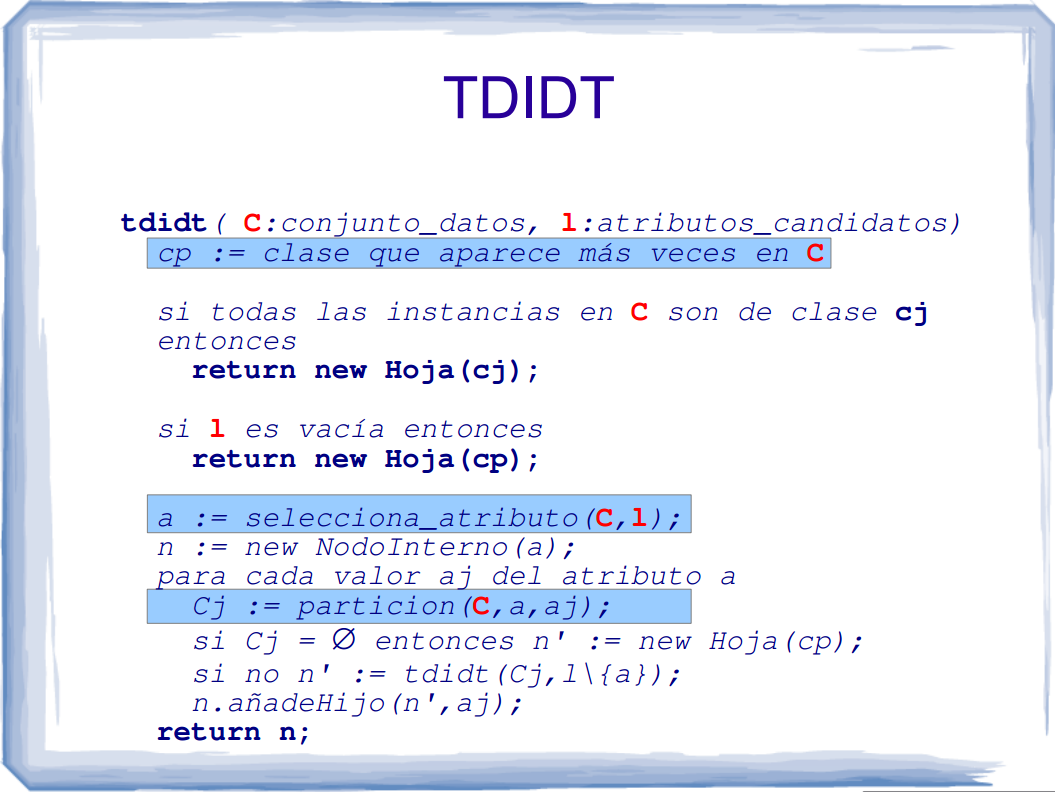
\includegraphics[width=\textwidth]{./images/esquemaTDIDT.png}
\end{frame}

\begin{frame}
  \frametitle{ID3\footnote{Diapositiva sacada del temario de SGDI}}
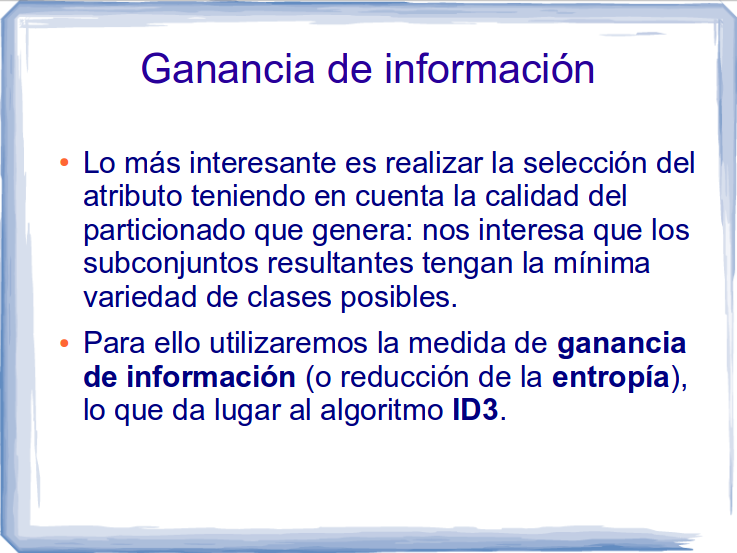
\includegraphics[width=\textwidth]{./images/esquemaID3.png}
\end{frame}

%=================================================
\sectionDark{C4.5}
%=================================================
\begin{frame}
  \frametitle{C4.5}
  El algoritmo ID3 es mejorado por el C4.5. Esta mejora, aparte de la
  optimizaci�n de partes de c�digo, incluye\footnote{Art�culo con las bases del algoritmo \cite{quinlan1986induction}}:
  \begin{itemize}
  \item Permite atributos continuos.
  \item Permite dar un peso diferente a cada atributo.
  \item Permite a una instancia no tener definido un valor en sus
    atributos.
  \item Mejora la selecci�n del atributo clasificador.
  \item Realiza una poda del �rbol despu�s de la creaci�n.
  \end{itemize}
\end{frame}

\begin{frame}[fragile]
  \frametitle{Algoritmo C4.5\footnote{Obtenido del libro \cite{quilan2014c4} y su review \cite{salzberg1994c4}}}
  \begin{tikzpicture}
    \tikzpicdimlarge
    \only<1->{\node[] (def) at (0.5,6) {
        \begin{minipage}{0.9\textwidth}
          \textcolor{purple}{\textbf{Funciones Test:}}
          Para calcular los subconjuntos de instancias al clasificar
          por un atributo se utilizan funciones test de tipo $x >
          40$ � $x < 4$ � $ x = soleado$.
        \end{minipage}
      };}

    \only<2->{\node[] (def) at (0.5,2) {
        \begin{minipage}{0.9\textwidth}
          \textcolor{purple}{\textbf{Selecci�n del atributo:}}
          La selecci�n del atributo por el que dividir consiste en
          escoger el atributo con mayor ganancia de informaci�n
          normalizado y ponderado. \\

          Para ello, se tiene en cuenta la proporci�n de instancias
          que queda en cada rama para el atributo candidato y el peso
          de importancia dado a dicho atributo.\\
          
          La f�rmula queda para el atributo $i$, siendo D el
          conjunto de instancias
          $$ Ganancia_i = Peso_i * \sum_j \frac{|D_j|}{|D|} * Info_j $$
        \end{minipage}
      };}

  \end{tikzpicture}
\end{frame}

\begin{frame}[fragile]
  \frametitle{Ejemplo --  ID3 vs C4.5 (atributos continuos)}
\begin{tikzpicture}
\tikzpicdimlarge
\only<1->{\node[] () at (0,9)
  {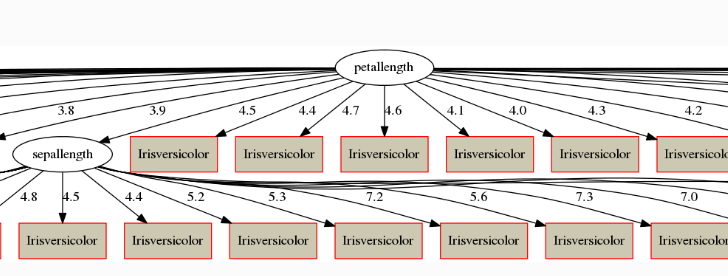
\includegraphics[width=0.65\textwidth]{images/ID3iris.png}};}
\only<2->{\node[] () at (0,5)
  {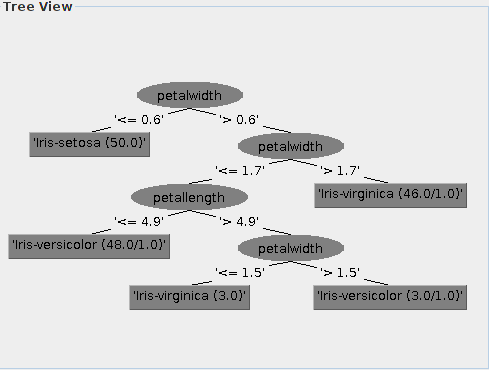
\includegraphics[width=0.65\textwidth]{images/C45tree.png}};}

\end{tikzpicture}
\end{frame}

\begin{frame}
  \frametitle{Mejoras a C4.5}

\end{frame}

%=================================================
\sectionDark{C5.0}
%=================================================

\begin{frame}
  \frametitle{C5.0}
% Mejoras
\end{frame}


%\begin{frame}
%  \frametitle{Ejemplo}
%\end{frame}

%===== EJEMPLO =====
%\begin{frame}[fragile] % Frame ejemplo 2
%  \frametitle{Ejemplo}
%\end{frame}



%=================================================
\sectionDark{Random Forest}
%=================================================
\begin{frame}
  \frametitle{Introducci�n -- I}
  \only<1>{\alert{Hasta ahora:}\\ \qquad Un conjunto de entrenamiento $\rightarrow$ Un �rbol
  de clasificaci�n\\}

  \only<2>{\alert{Random forest:}\\ \qquad Un conjunto de entrenamiento $\rightarrow$ Varios �rboles
    de clasificaci�n\\}

  \vspace{0.3cm}

  \begin{columns}
    \begin{column}{0.5\textwidth}
      \begin{tabular}{ccccc}
        Sexo & Altura & Peso & Exp. & Act. \\ \hline
        H & 1,55 & 45 & A+ & F�tbol \\
        H & 1,67 & 58 & C & F�tbol \\
        M & 1,45 & 45 & B & F�tbol \\
        M & 1,58 & 50 & A+ & P�del \\
        H & 1,20 & 40 & B & F�tbol \\
        M & 1,80 & 60 & A & P�del \\
        $\cdots$ & $\cdots$ & $\cdots$ & $\cdots$ & $\cdots$ \\ \hline
      \end{tabular}
    \end{column}
    \begin{column}{0.5\textwidth}
      \vspace{0.3cm}
      \includegraphics<1>[width=\textwidth]{images/randomForest/1arbol.png}
      \includegraphics<2->[width=\textwidth]{images/randomForest/bosque.png}
    \end{column}
  \end{columns}

\end{frame}


\begin{frame}
  \frametitle{Introducci�n -- II}

  \begin{block}{Random forest\footnote{T�cnica propuesta por primera vez en \cite{randomForest}.} (\textcolor{red}{No me gusta este t�tulo})}
    \begin{itemize}
    \item �C�mo se clasifica una instancia?
    \item �C�mo se generan varios �rboles con el mismo conjunto de
      entrenamiento?
    \item �C�mo se genera un �rbol en concreto?
    \end{itemize}
  \end{block}

   
\end{frame}


\begin{frame}[fragile,fragile]
  \frametitle{Clasificaci�n de instancias}
  
  Al existir varios �rboles, pueden existir varias clases posibles para una
  instancia.\\
  \quad La clase final ser� aquella que m�s veces aparece elegida (\alert{moda}).
\begin{lstlisting}[frame=single, numbers=left]
clasifica(x):
  for_each a in arboles:
     cjto += clasifica(x, a)

  return moda(cjto)
\end{lstlisting}

\begin{columns}
  \begin{column}{0.6\textwidth}
    \flushright
    \includegraphics<1>[scale=0.2]{images/randomForest/arbol_class1.png}
    \includegraphics<2->[scale=0.2]{images/randomForest/arbol_class2.png}
  \end{column}
  \begin{column}{0.4\textwidth}
    \includegraphics<-2>[scale=0.2]{images/randomForest/nodo.png}
    \includegraphics<3->[scale=0.2]{images/randomForest/nodo_naranja.png}
  \end{column}
\end{columns}

\end{frame}


\begin{frame}[shrink]
  \frametitle{Generaci�n de �rboles --- Selecci�n de instancias}
  \alert{Problema:} A partir de un mismo conjunto de entrenamiento se
  desean obtener distintos �rboles de clasificaci�n.\\
  \vspace{\baselineskip} % hack chapuza para meter una linea entre p�rrafos
  \alert{Soluci�n:}
  T�cnica conocida como \textbf{Bagging} o \emph{Bootstrap aggregating}:
  \begin{itemize}
  \item Dado un conjunto de entrenamiento con $N$ instancias, obtener $B$
    conjuntos de entrenamiento de tama�o $n'$ ($n' < N$).
  \item Utilizar \textit{muestreo aleatorio con reemplazamiento}.
  \end{itemize}

  \includegraphics<1>[width=\textwidth]{images/randomForest/bagging_pre.png}
  \includegraphics<2->[width=\textwidth]{images/randomForest/bagging.png}

\end{frame}


\begin{frame}[t]
  \frametitle{Generaci�n de �rboles --- Selecci�n de atributos}
  \onslide<1->{
    -- En un nodo split, �qu� atributo escoger para hacer la divisi�n? --\\
    \vspace{\baselineskip}
  }
  
  \only<1>{
    \textbf{ID3:} Escoger entre \texttt{todos} los atributos, aquel que
    proporcione una mayor ganancia de informaci�n.\\
    \vspace{\baselineskip}
    \alert{Problemas:} 
    \vspace{-0.5\baselineskip}
    \begin{itemize}
    \item Un atributo muy decisivo en un �rbol seguramente tambi�n lo sea en
      el resto de �rboles, por lo que producir�a �rboles muy correlacionados.
    \item Comparar entre todos los atributos en todos los �rboles necesita
      muchos recursos.
    \end{itemize}
  }

  \only<2->{
    \alert{Soluci�n:} \textbf{Feature bagging}\footnote{Descrita
      principalmente en~\cite{FeatureBagging}}
    \begin{itemize}
    \item En cada nodo split, observar solamente un subconjunto aleatorio
      de tama�o $m'$ del conjunto de atributos restantes.
    \item Sobre el subconjunto, escoger el que mayor ganancia de
      informaci�n proporcione (similar a ID3).
    \item Si el n�mero de atributos totales es $m$, el subconjunto de
      tama�o $m'$ se calcula de manera aleatoria, donde:\\
$$
      m' =
      \left\{
	\begin{array}{ll}
          \lfloor \sqrt{m} \rfloor  & \mbox{si } \sqrt{m} \geq 5 \\
          m &  c.c.
	\end{array}
      \right.
$$
\end{itemize}
  }

  
\end{frame}

%
%
%%%
%%% Local Variables:
%%% mode: latex
%%% TeX-master: "PRESENTACION.tex"
%%% End:




%======= BIBLIOGRAF�A =======
\begin{frame}
  \frametitle{Bibliograf�a}
  
  \begin{enumerate}
  \item \textbf{Wikipedia:}\\\url{https://en.wikipedia.org/}
  \end{enumerate}
\end{frame}

\end{document}
